\chapter{File Carving}
File Carving é o processo de recuperação de fragmentos de arquivos não mais indexados baseado no seu conteúdo e na ausência de metadados do sistema de arquivos \cite{BinCarver}. 

O processo de File Carving é útil na recuperação de arquivos e amplamente utilizado em investigações digitais (em forense computacional). Devido a isso, esse é um dos processos mais importantes e desafiadores da computação forense \cite{DGI}.

Um dos primeiros desafios do processo de file carving, segundo Memon (2008, p. S2), se encontra na tentativa de se recuperar arquivos fragmentados. Um ponto chave no processo de recuperação desses arquivos fragmentados é encontrar a relação de fragmentação do arquivo que pode beneficiar o processo de recuperação de dados. Técnicas tradicionais não conseguem recuperar arquivos quando o sistema de arquivos é ou está corrompido, quando a tabela de alocação não está presente ou possui endereçamentos errados ou incompletos. Assim, a técnica de File Carving apresenta sua capacidade de recuperar arquivos em espaços não alocados do disco (área do disco não apontada pela tabela de partição - no caso do NTFS, a Master File Table).

\section{Assinatura de Arquivo}
As ferramentas de file carving mais comuns analisam as informações de assinatura do arquivo, através do cabeçalho e do rodapé do arquivo, determinando assim o conteúdo do arquivo entre esses blocos. Infelizmente, ferramentas poderosas de file carving atuais ainda falham na recuperação de arquivos fragmentados.

\section{Arquivos Fragmentados}
Segundo Kloe (2007, p. 8), um arquivo fragmentado é um arquivo dividido em várias partes onde cada parte pode estar localizada em um lugar diferente em um mesmo conjunto de dados. Sistemas operacionais modernos, tais como o NTFS, tentam gravar os dados evitando a fragmentação porém, ainda existem algumas situações em que a fragmentação ocorre. Já Memon define que um arquivo é dito fragmentado quando o mesmo está armazenado de forma descontinuada nos clusters, e que o maior desafio para o processo de data carving é justamente a recuperação de arquivos quando esses estão fragmentados em duas ou mais partes. 

Garfinkel (2007, p. S4) defendia a hipótese de que diferentes tipos de arquivos poderiam apresentar diferentes padrões de fragmentação, o que poderia determinar uma fragmentação diferenciada para um tipo de arquivo específico no disco. Arquivos comumente de sistemas, instalados juntamente com a parte do sistema operacional apresentariam um baixo fator de fragmentação enquanto arquivos comuns e altamente importantes na análise forense, por se tratarem de informações do dia a dia tais como documentos (.doc), mídias (.avi, .jpeg), arquivos de correio eletrônico armazenados (.pst), planilhas com cálculos e fórmulas (.xls), arquivos de log e arquivos texto (.txt), aparentam ter uma tendência a maior fragmentação se comparados à arquivos menos significativos para o processo forense. Garfinkel (2007, p. S2) então chegou a uma das principais conclusões, que até 42\% de arquivos de e-mail (.pst), 17\% de arquivos microsoft word (.doc) e 16\% de arquivos de imagem (.jpeg) são fragmentados, deixando bem claro que a 
recuperação de arquivos fragmentados é um problema crítico para a análise forense. Outro fator importante que tem influencia a fragmentação, que pode ser percebido por Garfinkel (2007, p. S6), é que em dispositivos com maior capacidade de armazenamento o fator de fragmentação é menor se comparado a dispositivos de menor capacidade de armazenamento.

\begin{itemize}
 \item Quando não há mais espaço de mídia suficiente na sequência física para a gravação de um arquivo, assim, para ser alocado no disco ele tem que ser dividido em dois ou mais fragmentos.
 \item Na sequência de um arquivo já alocado, o espaço restante no cluster não é suficiente para a gravação do arquivo sequencialmente, sendo necessária a divisão do arquivo em dois ou mais fragmentos.
\end{itemize}

\subsection{Fragmentação Linear}
Kloe referencia a fragmentação linear a arquivos que estão fragmentados seguindo a sequência original no disco. A figura \ref{fig:fraglinear} demonstra a fragmentação linear na ordem original do disco.

\begin{figure}[htp]
  \centering
  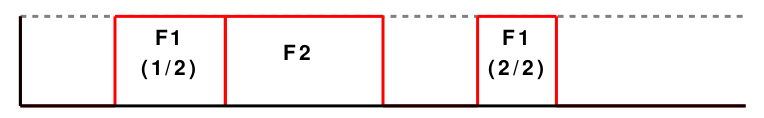
\includegraphics[scale=0.6]{figuras/fraglinear.png}
  \caption{Exemplo de Fragmentação Linear}
  \label{fig:fraglinear}
\end{figure}

\subsection{Fragmentação Não Linear}
Conforme Kloe, a fragmentação não linear representa os arquivos fragmentados fora da ordem normal de sequência do disco. A figura \ref{fig:fragnaolinear} demonstra como os fragmentos do arquivo F1 estão fora da sequência natural do disco.

\begin{figure}[htp]
  \centering
  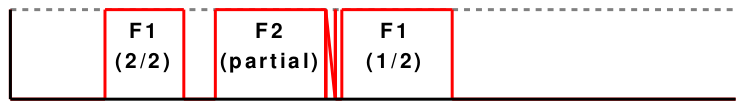
\includegraphics[scale=0.6]{figuras/fragnaolinear.png}
  \caption{Exemplo de Fragmentação Não Linear}
  \label{fig:fragnaolinear}
\end{figure}

\subsection{Arquivo Parcial}
A figura \ref{fig:fragnaolinear} demonstra não somente a fragmentação não linear mas também a sobreposição de parte do arquivo. Isso demonstra um arquivo não mais alocado que fora parcialmente sobrescrito. O arquivo pode nunca mais ser totalmente recuperado porém, parte da informação útil do arquivo ainda está presente na área antes alocada para o mesmo. Kloe diz que para o processo de carving não há diferença entre uma informação parcial e um arquivo fragmentado que ainda não tenha sido totalmente recuperado. Um primeiro detalhe sobre a afirmação de Kloe é que um dos arquivos pode ser totalmente recuperado dependendo do tempo e da profundidade de busca da ferramenta de carving (em algum momento conseguiria encontrar as demais partes do arquivo), enquanto um arquivo parcial (sobrescrito) não possui mais suas partes perdidas (por terem sido sobrescritas) no disco e que a ferramenta de carving em algum momento terá que definir se tratar de um arquivo parcial.

\subsection{Recuperação de Arquivos Fragmentados}
Para recuperar arquivos fragmentados, qualquer ferramenta de file carving precisa ser capaz de identificar o ponto de início do arquivo e os blocos necessários para reconstruir o arquivo. Segundo Memon (2008, p. S4), há basicamente três pontos a se seguir no processo de carving:

\begin{enumerate}
 \item Identificar o ponto inicial do arquivo.
 \item Identificar os blocos pertencentes ao arquivo.
 \item Organizar os blocos de forma correta para que se possa reconstruir o arquivo.
\end{enumerate}

[PAREI AQUI!!!!!!!]

\section{Aspectos de Carving}

\subsection{Cabeçalho e Rodapé}
Atualmente a simples comparação byte por byte é uma operação muito rápida que computadores atuais podem processar com facilidade. Sendo assim, a verificação de cabeçalhos e rodapés estáticos de tipos de arquivos se torna um dos primeiros passos que um algoritmo de recuperação pode seguir. Com base nas informações contidas no cabeçalho e rodapé de um arquivo pode-se determinar o tipo do arquivo em questão e até mesmo, em alguns casos, informações mais específicas referentes ao arquivo (metadados\footnote{Informação descritiva sobre um dado ou um item, metainformação}) \cite{DGI}.

A análise de cabeçalho e rodapé é a técnica mais básica de carving. A técnica consiste em procurar no conjunto de dados por padrões que definem o início do bloco de um arquivo, como por exemplo o cabeçalho de um arquivo de imagem (.png) demonstrado pela figura \ref{fig:png-file-format} \cite{Kloet}.

\begin{figure}[htp]
  \centering
  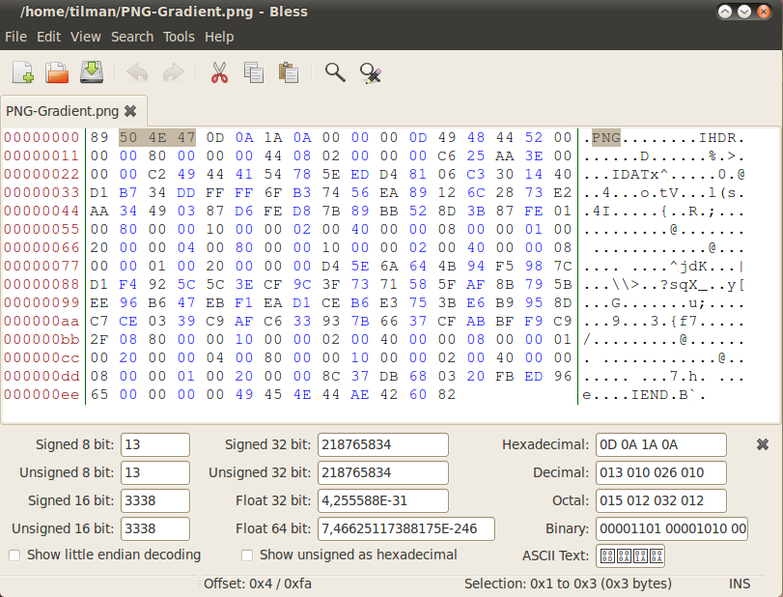
\includegraphics[scale=0.5]{figuras/png-file-format.png}
  \caption{Estruda de cabeçalho de um arquivo do tipo PNG \cite{PngFileFormat}}
  \label{fig:png-file-format}
\end{figure}

O valor hexadecimal ``89  50  4e  47  0d  0a  1a  0a'' representa os 8 bytes do cabeçalho de arquivos PNG. Cada arquivo PNG é marcado a partir desse cabeçalho. A marca final do arquivo ou o rodapé do arquivo delimita o final do arquivo. O conteúdo entre o cabeçalho do arquivo e o final do arquivo seria a representação da informação do arquivo \ref{fig:png-file-structure-data}.

\begin{figure}[htp]
  \centering
  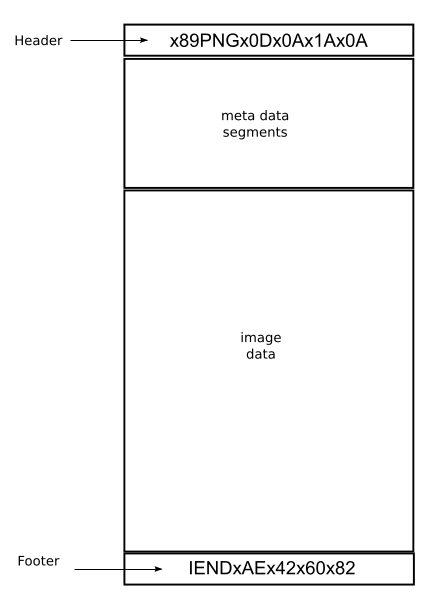
\includegraphics[scale=0.6]{figuras/png-file-structure-data.png}
  \caption{Área de dados de um arquivo do tipo PNG \cite{Kloet}}
  \label{fig:png-file-structure-data}
\end{figure}

Segundo Kloet (2007, p. 9), a análise de cabeçalho e rodapé é um método que apresenta alguns problemas relevantes:

\begin{itemize}
 \item Muitos falsos positivos.
 \item Incapacidade de detectar arquivos fragmentados e arquivos parciais.
 \item Alguns arquivos não apresentam cabeçalho fixo, assim como alguns arquivos também apresentam rodapé variável, o que impossibilita sua identificação por esse método.
\end{itemize}

O mesmo ocorre para o método de cabeçalho com tamanho máximo possível de dados, técnica que visa recuperar os dados pelo comprimento máximo disposto para o tipo de arquivo para sua área de dados. Além desses os problemas da técnica de cabeçalho e rodapé, esta técnica ainda tem outros dois problemas ligados à área de dados. Tendo em vista que a área máxima não é exatamente a área máxima estipulada pela definição do tipo de arquivo e sim uma questão de referência, esses dados podem ser primeiramente coletados além do tamanho real do arquivo no dispositivo de origem como também poderá ser menor que o próprio tamanho dos dados do arquivo no dispositivo de origem.

\subsection{Carving em Estrutura de Arquivo}
...

\section{Número Mágico}
...